\documentclass[11pt]{article}
\usepackage[utf8]{inputenc}
\usepackage{hyperref}
\hypersetup{
    colorlinks=true,
    linkcolor=blue,
    filecolor=magenta,      
    urlcolor=cyan,
}

\title{Projektmanagement-Plan - Message Logger \\
	Team 4}
\author{Stephan Stofer\\
	Maurizio Hostettler\\
	Julien Grüter\\
	Adrian Willi\\}
\date{Frühlingssemester 2020 \\
Version 2.0.0}

\usepackage{natbib}
\usepackage{graphicx}
\usepackage[a4paper, left=2cm, right=2cm, top=2cm, bottom=2cm]{geometry}
\usepackage{booktabs}
\usepackage[table,xcdraw]{xcolor}
\begin{document}

\maketitle

\begin{table}[]
	\centering
	\begin{tabular}{|l|l|l|l|l|}
		\hline
		\textbf{Rev}   & \textbf{Datum} & \textbf{Autor} & \textbf{Bemerkungen} & \textbf{Status} \\ \hline
		1.0.0 & 19.04.2020 & Alle  & 1. Version - Zwischenabgabe & Fertig \\ \hline
		1.0.1 & 20.04.2020 & Alle & Überarbeitete 1. Version gemäss Feedback Zwischenabgabe                             & Fertig        \\ \hline
		1.0.2 &	17.05.2020 & Alle & Überarbeitete Version gemäss Review & Fertig        \\ \hline
		2.0.0 &	18.05.2020 & Alle & Schlussabgabe & Fertig        \\ \hline
	\end{tabular}
\end{table}

\newpage 
\tableofcontents{}
\newpage

\section{Projektorganisation}
\subsection{Projektauftrag}
Es soll eine Logger-Komponente für ein Spiel entwickelt werden. Bei der Logger-Komponente handelt es sich um eine Software-Komponente, die einfach in bestehende Java-Applikationen eingebunden werden kann. Eine Applikation kann durch einfache Methodenaufrufe Meldungen (Messages) über die Logger-Komponente dauerhaft aufzeichnen. Die Meldungen aller Applikationen sollen in einem zentralen Logger Server in einem wohldefinierten Format gespeichert werden. Über den LoggerViewer können die geloggten Nachrichten auf dem LogServer in einem GUI angezeigt werden.

\begin{center}
	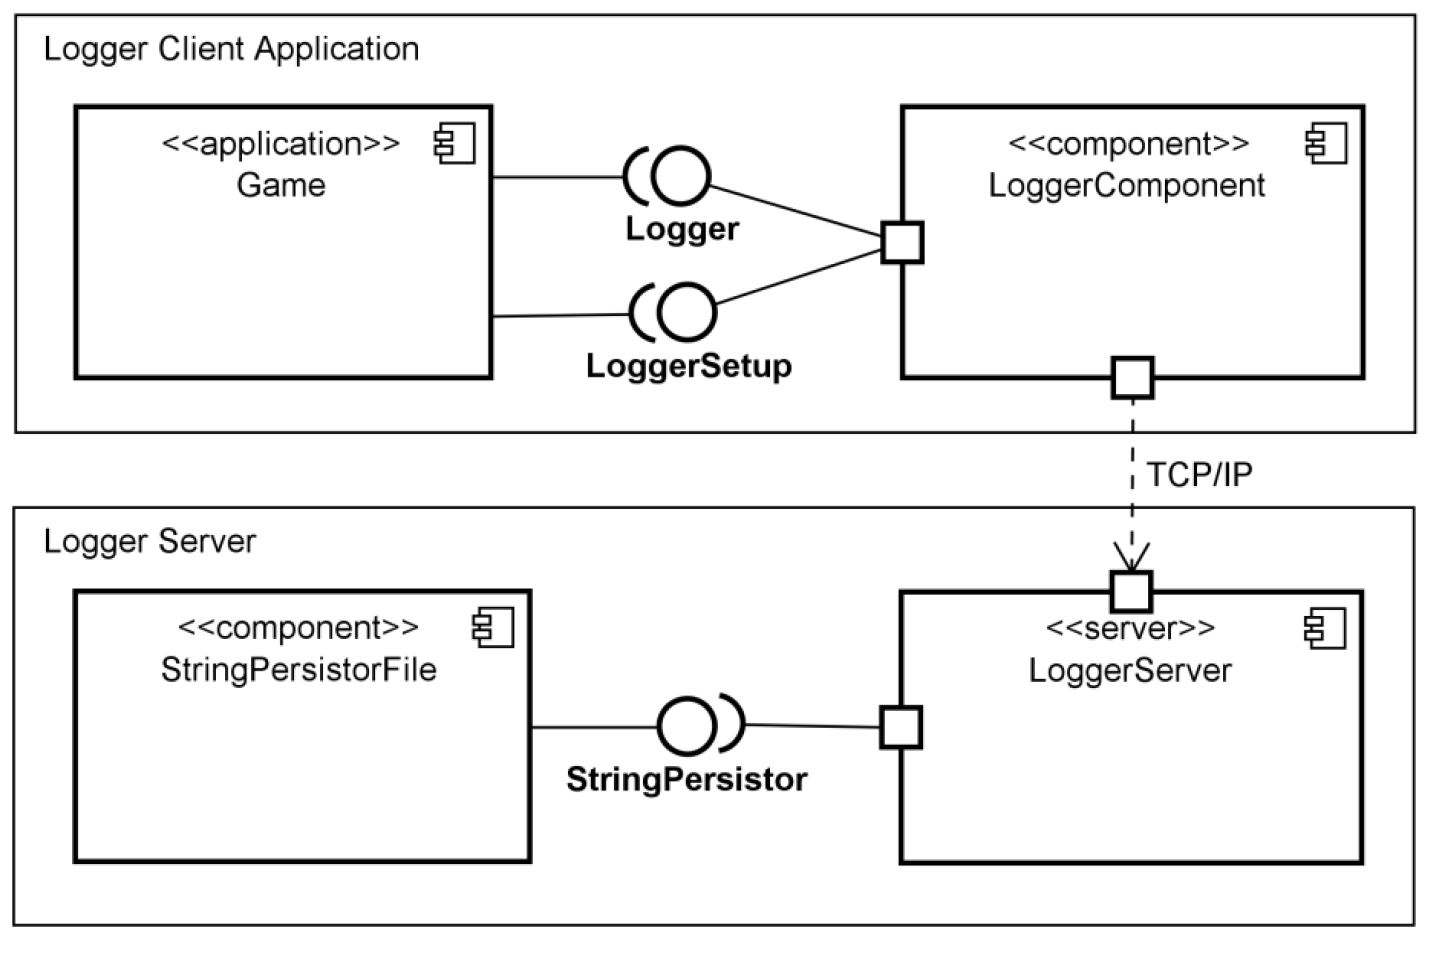
\includegraphics[height=8cm,keepaspectratio]{images/Logger.JPG}
\end{center}

\subsection{Projektmanagement}
\subsubsection{Organigramm}
\begin{center}
	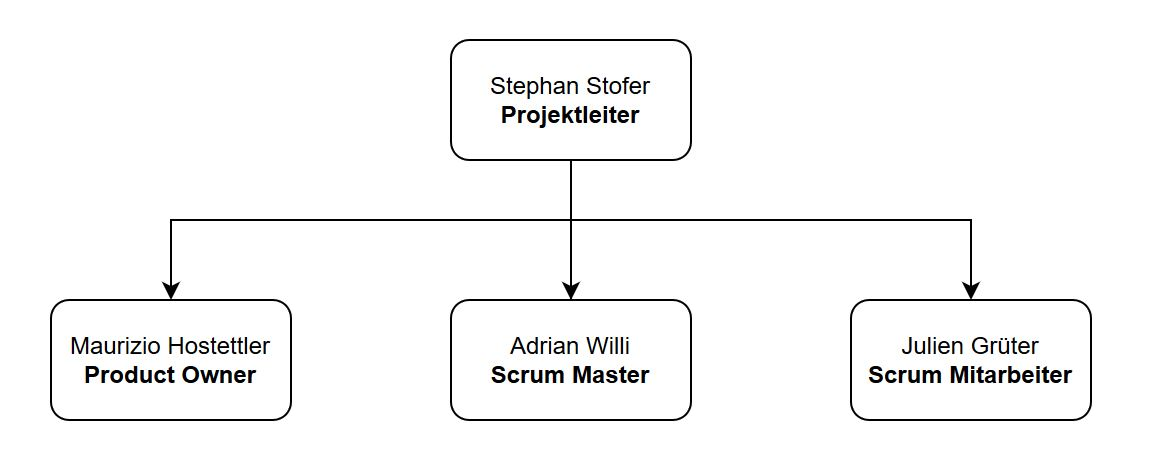
\includegraphics[height=6cm,keepaspectratio]{images/Organisation.JPG}
\end{center}

\subsubsection{Rollen und Zuständigkeiten}
\begin{itemize}
	\itemsep0pt
	\item \textbf{Stephan Stofer - Projektleiter / Scrum Mitarbeiter: }Der Projektleiter wird in der Initialisierungs- und Einführungsphase eine Schlüsselrolle einnehmen. Der Fokus seiner Tätigkeit wird in der Organisation des Projektes sowie in der Erstellung eines Rahmenplans liegen. Diser Rahmenplan gibt eine grobe Vorstellung des übergeordneten Projektablaufs mit den wichtigsten Meilensteinen und Terminen.
	\item \textbf{Maurizio Hostettler - Product Owner / Member Interface-Komitee / Scrum Mitarbeiter: }Der Product Owner wird in der Konzeptions- und Realisierungsphase eine entscheidende Rolle einnehmen. Seine Haupttätigkeit umfasst die Product Backlog-Pflege und -Priorisierung sowie die Sprint-Planung und -Abnahme. Als Zusatzfunktion wird er innerhalb der Gruppe noch als Member des Interface-Komitees agieren.
    \item \textbf{Adrian Willi - Scrum Master / Scrum Mitarbeiter: }Der Scrum Master ist in jeder Phase des Projekts essentiell. Er wird als Vermittler zwischen dem Scrum Team und dem Product Owner agieren. Zudem unterstützt er ein korrektes Projektvorgehen und stellt die Qualität der Leistung sicher.
    \item \textbf{Julien Grüter - Scrum Mitarbeiter: }Er wird bei der Entwicklung eine wichtige Rolle spielen und kann dort seine Erfahrungen aus der Praxis einfliessen lassen. Er wird auch sicherstellen, dass der Code den Anforderungen entspricht und andere Teammitglieder bei Bedarf unterstützen bei Ihren Tätigkeiten.
\end{itemize}

\subsubsection{Projektstrukturplan}
Auf einen Projektstrukturplan wird explizit verzichtet, da das Projekt klein ist und sonst nur ein unnötiger Overhead entsteht.


\section{Projektführung}
Das Projektmanagement in diesem Projekt wird mit der Projektmethode SoDa gemacht.
\subsection{Rahmenplan}
Hierbei handelt es sich um einen aktualisierten Rahmenplan. Die Änderungen wurden ausgelöst durch die Umstellung auf reinen Onlineunterricht.



\begin{center}
	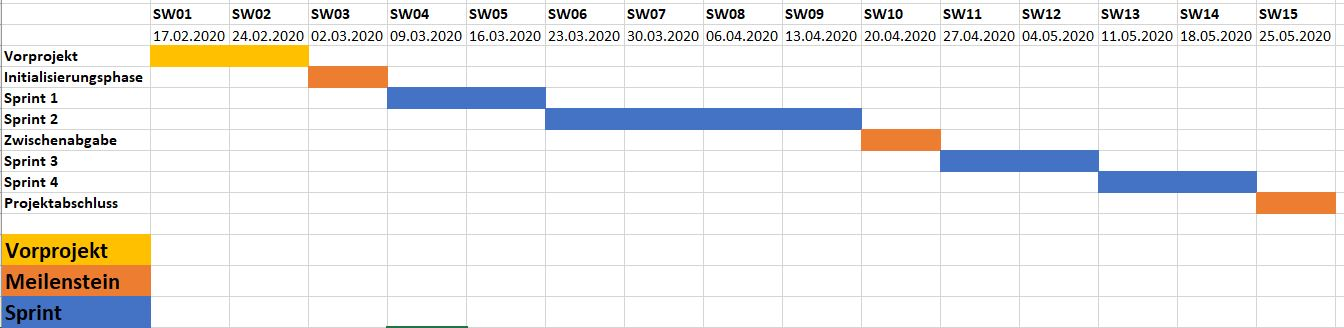
\includegraphics[height=4.5cm,keepaspectratio]{images/Projektrahmenplan_2V.JPG}
\end{center}
Wichtige Daten:
\begin{itemize}
	\itemsep0pt
	\item \textbf{Meilensteine: }
	\begin{itemize}
		\itemsep0pt
		\item Meilenstein 1: SW03 (02.03.2020)
		\item Meilenstein 2: SW10 (20.04.2020)
		\item Meilenstein 3: SW15 (25.05.2020)
	\end{itemize}
	
	\item \textbf{Sprints: }
		\begin{itemize}
		\itemsep0pt
		\item Sprint 1: SW04 - SW05
		\item Sprint 2: SW06 - SW09
		\item Sprint 3: SW11 - SW12
		\item Sprint 4: SW13 - SW14
	\end{itemize}
\end{itemize}



\subsection{Projektkontrolle}
Die Projektkontrolle wird im  \href{https://gitlab.enterpriselab.ch/vsk-20fs01/g04/g04-project/boards}{Gitlab} geführt und ist dort ersichtlich.

\subsection{Meilensteinplanung}
Die Meilensteinplanung wurde auf Basis des Rahmenplans erstellt. Das Projekt gliedern wir in 3 Meilensteine. Dabei ist zu Beginn, in der Mitte des Projektes sowie am Ende ein Meilenstein vorgesehen. Die Meilensteine richten sich an den Vorgaben des Auftragsgebers aus. Im Anhang sind die Ziele und Reviews der Meilensteine ersichtlich in Form von Meilensteinberichten. 
\subsection{Sprintplanung}
Die Sprintplanung ist eine rollende Detailplanung. Der Product Owner priorisiert laufend, zusammen mit dem Entwicklungsteam und dem Auftraggeber, die Epic, respektive die User Stories im Backlog. Zusammen mit dem Entwicklungsteam schätzt der Product Owner den Aufwand der höchst priorisierten Anforderungen und setzt diese im folgenden Sprint um. Die Sprintdauer umfasst im Normalfall 2 Wochen, wobei Abweichungen natürlich möglich sind. \\ 
Die Aufwandschätzungen in der einzelnen Stories werden jeweils nach Personentagen im GitLab vorgenommen. \\
Im Anhang sind der Product Backlog, Sprintplanungen, Sprintreviews sowie Retrospektiven ersichtlich. Die einzelenen Item und Sprints sind ebenfalls im  \href{https://gitlab.enterpriselab.ch/vsk-20fs01/g04/g04-project/boards}{Gitlab} ersichtlich. 

\subsubsection{Definition of Done}
\begin{center}
	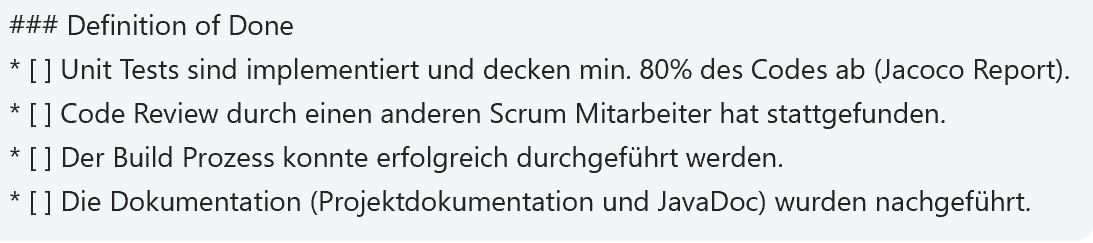
\includegraphics[height=4cm,keepaspectratio]{images/Dod.JPG}
\end{center}
Diese Definition wird im GitLab bei jedem Issue hinzugefügt und entsprechend angepasst. Speziell werden die spezifischen Akzeptanzkriterien jeweils festgehalten.

\subsection{Risikomanagement}
Im Rahmen der Risikoanalyse haben wir folgende Risiken identifiziert:
\subsubsection{Unvorhergesehene Anforderungsänderungen während eines Sprints}
Anforderungen an Komponenten oder Interface ändern sich während Entwicklungszyklen fundamental.
\paragraph{Massnahmen zur Risikominderung}
\begin{itemize}
\item Falls Probleme oder Unsicherheiten entstehen, sind diese sofort mit den anderen Team-Mitglieder zu besprochen. (Eintrittswahrscheinlichkeit minimieren)
\item Pro Sprint einen halben Tag Pufferzeit einplanen. (Eintrittswahrscheinlichkeit minimieren)
\end{itemize}

\subsubsection{Ausfall Projektmitglied}
Ausfall eines Projektmitglieds durch Unfall oder Krankheit.
\paragraph{Massnahmen zur Risikominderung}
\begin{itemize}
\item Regelmässiger Austausch mit den Mitgliedern, um über den jeweils aktuellen Stand zu informieren (Auswirkung minimieren)
\item Gitlab sowie die Dokumentation auf dem aktuellen Stand halten (Auswirkung minimieren)
\item Gesunde Ernährung mit viel Gemüse und Früchten (Eintrittswahrscheinlichkeit minimieren)
\item Ausreichend Schlaf und genügend Pausen während längeren Arbeitsphasen (Eintrittswahrscheinlichkeit minimieren)
\end{itemize}
\subsubsection{Ungleiche Arbeits-/Wissensverteilung in Projektgruppe}
Aufgaben und oder Wissen über Projektfortschritte unregelmässig in Projektgruppe verteilt.
\paragraph{Massnahmen zur Risikominderung}
\begin{itemize}
\item Weekly MeetUp vor oder nach der Vorlesung in dem wir uns über das Projekt, Projektstand sowie Aufgaben während der Woche austauschen (Auswirkung minimieren)
\item Sprintplan in \href{https://gitlab.enterpriselab.ch/vsk-20fs01/g04/g04-project/boards}{Gitlab} ist von allen Mitgliedern regelmässig prüfen (Auswirkung minimieren)
\item Regelmässiger Austausch mit den Mitgliedern, um über den jeweils aktuellen Stand zu informieren (Auswirkung minimieren)
\item Gitlab sowie die Dokumentation auf dem aktuellen Stand halten (Auswirkung minimieren)
\item Austausch bei Fragen oder Problemen ausserhalb des Vorlesungsblocks findet über WhatsApp-Gruppenchat statt (Auswirkung minimieren)
\end{itemize}
\subsubsection{Mangelhafte Professionalität der Projektmitarbeiter}
Mangelhafte Codequalität und oder fehlerhafter Einsatz von Entwicklungswerkzeuge wie IDE und Git. Unprofessionelles Verhalten der Projektmitarbeiter.
\paragraph{Massnahmen zur Risikominderung}
\begin{itemize}
\item Regelmässige Code-Review welche selbstständig zu organisieren sind (Eintrittswahrscheinlichkeit minimieren)
\item Befolgen der Clean Code Leitlinien und automatisierte Überprüfung der Qualität mittels Jenkins (Eintrittswahrscheinlichkeit minimieren)
\item Für die Entwicklungswerkzeuge sollen jeweils im README die wichtigsten Befehle festgehalten werden, damit alle gleich mit den Werkzeugen arbeiten.  (Eintrittswahrscheinlichkeit minimieren)
\item Selbstständiges Einarbeiten in IDE und Git (Eintrittswahrscheinlichkeit minimieren)
\item Regelmässige Datensicherung mit TimeMachine oder ähnlichen Dienstprogrammen (Auswirkung minimieren)
\item Einsatz aktueller Virensoftware und regelmässiges aktualisieren der Datenbanken auf allen Arbeitsgeräten (Eintrittswahrscheinlichkeit minimieren)
\end{itemize}
\subsubsection{COVID-19}
Der Coronavirus könnte sich jederzeit auch in Europa und somit in der Schweiz verbreiten. Dies könnte unter Umständen, zu einer Schliessung der Schulen führen, wie dies bereits in Asien geschehen ist.
\paragraph{Massnahmen zur Risikominderung}
\begin{itemize}
\item Im Falle einer Schliessung der Schule, wird das Team weiterhin eng zusammenarbeiten (Eintrittswahrscheinlichkeit minimieren)
\item Verstärkter Nutzen der gängigen Kommunikationstools wie Skype oder WhatsApp (Eintrittswahrscheinlichkeit minimieren)
\end{itemize}





\section{Projektunterstützung}
\subsection{Tools für Entwicklung, Test und Abnahme}
Im Projektmanagement setzen wir folgende Tool ein:
\begin{table}[!h]
	\resizebox{\textwidth}{!}{%
		\begin{tabular}{@{}llll@{}}
			\toprule
			\rowcolor[HTML]{C0C0C0} 
			Bereich                 & Tool\\ \midrule
			\multicolumn{1}{|l|}{Vorgehensmodell: SoDa}  & \multicolumn{1}{l|}{GitLab}          \\ \midrule
			\multicolumn{1}{|l|}{Datenaustausch}  & \multicolumn{1}{l|}{GitLab, OneDrive}     \\ \midrule
			\multicolumn{1}{|l|}{Kommunikation}  & \multicolumn{1}{l|}{WhatsApp, Skype, Zoom}     \\ \midrule
			\multicolumn{1}{|l|}{Dokumentation} & \multicolumn{1}{l|}{Microsoft Office, Draw.io, yFiles}\\ \bottomrule
			
		\end{tabular}%
	}
\end{table} 
In der Entwicklung setzen wir folgende Tool ein:
\begin{table}[!h]
	\resizebox{\textwidth}{!}{%
		\begin{tabular}{@{}llll@{}}
			\toprule
			\rowcolor[HTML]{C0C0C0} 
			Bereich                 & Tool\\ \midrule
			\multicolumn{1}{|l|}{Entwicklungsumgebung}  & \multicolumn{1}{l|}{IntelliJ IDEA, Eclipse, VS Code}          \\ \midrule
			\multicolumn{1}{|l|}{Programmiersprache}  & \multicolumn{1}{l|}{Java}     \\ \midrule
			\multicolumn{1}{|l|}{Versionskontrolle}  & \multicolumn{1}{l|}{GitLab}     \\ \midrule
			\multicolumn{1}{|l|}{Testing}  & \multicolumn{1}{l|}{JUnit, Integrations- und Systemtests}     \\ \midrule
			\multicolumn{1}{|l|}{Build}  & \multicolumn{1}{l|}{Maven}     \\ \midrule
			\multicolumn{1}{|l|}{Continuos Integration} & \multicolumn{1}{l|}{Jenkins}\\ \bottomrule
			
		\end{tabular}%
	}
\end{table}
\newpage
\subsection{Konfigurationsmanagement}
Das Konfigurationsmanagement soll die Einhaltung von Regeln für einen organisatorischen und verhaltensmässigen Lebenslauf eines Produkts und seiner Configuration Items (Konfigurationseinheiten) gewährleisten.
Ein Configuration Item ist eine beliebige Kombination aus Hardware, Software und / oder Dienstleistung. In diesem Projekt sind das die Dokumentationen, Komponenten und Interfaces. Im Kapitel Releasemanagement sind eben erwähnte ausführlich aufgelistet.
\subsection{Releasemanagement}
Das Releasemanagement befasst sich mit der Planung und Durchführung der Veröffentlichung. Dieses Projekt beinhaltet zwei Releases:
\begin{itemize}
\itemsep0pt
\item \textbf{Release 1:}Zwischenabgabe (SW10)
\item \textbf{Release 2:}Schlussabgabe (SW14)
\end{itemize}
\begin{table}[!h]
	\resizebox{\textwidth}{!}{%
		\begin{tabular}{@{}llll@{}}
			\toprule
			\rowcolor[HTML]{C0C0C0} 
			Configuration Item & Release 1                 & Release 2\\ \midrule
			\multicolumn{1}{|l|}{Projektmanagementplan}  & \multicolumn{1}{l|}{1.0.0}  & \multicolumn{1}{l|}{1.0.2}        \\ \midrule
			\multicolumn{1}{|l|}{Systemspezifikation}  & \multicolumn{1}{l|}{1.0.0} & \multicolumn{1}{l|}{1.0.2}    \\ \midrule
						\multicolumn{1}{|l|}{Testplan}  & \multicolumn{1}{l|}{1.0.0} & \multicolumn{1}{l|}{1.1.0}    \\ \midrule
			\multicolumn{1}{|l|}{GameOfLife}  & \multicolumn{1}{l|}{1.0.0-SNAPSHOT}& \multicolumn{1}{l|}{1.0.0-SNAPSHOT}     \\ \midrule
			\multicolumn{1}{|l|}{Logger}  & \multicolumn{1}{l|}{1.0.0}& \multicolumn{1}{l|}{1.0.0}     \\ \midrule
			\multicolumn{1}{|l|}{LoggerSetup}  & \multicolumn{1}{l|}{1.0.0}& \multicolumn{1}{l|}{1.0.0}     \\ \midrule
			\multicolumn{1}{|l|}{LoggerCommon}  & \multicolumn{1}{l|}{1.0.0-SNAPSHOT}& \multicolumn{1}{l|}{1.0.0-SNAPSHOT}     \\ \midrule
			\multicolumn{1}{|l|}{LoggerComponent}  & \multicolumn{1}{l|}{1.0.0-SNAPSHOT}& \multicolumn{1}{l|}{1.0.0-SNAPSHOT}     \\ \midrule
			\multicolumn{1}{|l|}{LoggerServer}  & \multicolumn{1}{l|}{1.0.0-SNAPSHOT}& \multicolumn{1}{l|}{1.0.0-SNAPSHOT}     \\ \midrule
			\multicolumn{1}{|l|}{LoggerClient}  & \multicolumn{1}{l|}{-}& \multicolumn{1}{l|}{1.0.0-SNAPSHOT}     \\ \midrule
			\multicolumn{1}{|l|}{StringPersistor}  & \multicolumn{1}{l|}{5.0.3}& \multicolumn{1}{l|}{5.0.3}     \\ \midrule
			\multicolumn{1}{|l|}{StringPersistorFile} & \multicolumn{1}{l|}{1.0.0-SNAPSHOT}& \multicolumn{1}{l|}{1.0.0-SNAPSHOT}\\ \bottomrule
			
		\end{tabular}%
	}
\end{table}
\newpage
\section{Teststrategie und -Drehbuch}
Teststrategie und Drehbuch sind in einem seperaten Dokument zu finden.

\section{Anhang}


\subsection{Product Backlog}
Das Product Backlog beinhaltet alle Anforderungen des Kunden. Diese werden laufend zusammen mit dem Product Owner ausgearbeitet und priorisiert. Vollständiger Backlog ist im GitLab ersichtlich.
\begin{table}[!h]
	\resizebox{\textwidth}{!}{%
		\begin{tabular}{@{}llll@{}}
			\toprule
			\rowcolor[HTML]{C0C0C0} 
			Issue ID                 & Titel                                                                          & Sprint                                     & Label                             \\ \midrule
			\multicolumn{1}{|l|}{1}  & \multicolumn{1}{l|}{Interface Definieren und Ausarbeiten}                      & \multicolumn{1}{l|}{Initialisierungsphase} & \multicolumn{1}{l|}{}             \\ \midrule
			\multicolumn{1}{|l|}{2}  & \multicolumn{1}{l|}{Projektdokumentation vorbereiten}                          & \multicolumn{1}{l|}{Initialisierungsphase} & \multicolumn{1}{l|}{}             \\ \midrule
			\multicolumn{1}{|l|}{3}  & \multicolumn{1}{l|}{Milesstones in Gitlab erfassen}                            & \multicolumn{1}{l|}{Initialisierungsphase} & \multicolumn{1}{l|}{}             \\ \midrule
			\multicolumn{1}{|l|}{4}  & \multicolumn{1}{l|}{ProduktBacklog Issues erfassen}                            & \multicolumn{1}{l|}{Initialisierungsphase} & \multicolumn{1}{l|}{}             \\ \midrule
			\multicolumn{1}{|l|}{5}  & \multicolumn{1}{l|}{Risikoanalyse}                                             & \multicolumn{1}{l|}{Initialisierungsphase} & \multicolumn{1}{l|}{}             \\ \midrule
			\multicolumn{1}{|l|}{7}  & \multicolumn{1}{l|}{Log Statements implementieren}                             & \multicolumn{1}{l|}{Sprint 1}              & \multicolumn{1}{l|}{Game-of-Live} \\ \midrule
			\multicolumn{1}{|l|}{8}  & \multicolumn{1}{l|}{Logger Interface implementieren}                           & \multicolumn{1}{l|}{Sprint 1}              & \multicolumn{1}{l|}{Game-of-Live} \\ \midrule
			\multicolumn{1}{|l|}{9}  & \multicolumn{1}{l|}{Logger Interface definieren}                               & \multicolumn{1}{l|}{Sprint 1}              & \multicolumn{1}{l|}{Logger}       \\ \midrule
			\multicolumn{1}{|l|}{10}  & \multicolumn{1}{l|}{Logger Klassen implementieren}                             & \multicolumn{1}{l|}{Sprint 1}                      & \multicolumn{1}{l|}{Logger}       \\ \midrule
			\multicolumn{1}{|l|}{11} & \multicolumn{1}{l|}{TCP/IP Kommunikation zu Log-Server implementieren}         & \multicolumn{1}{l|}{Sprint 2}                      & \multicolumn{1}{l|}{Logger}       \\ \midrule
			\multicolumn{1}{|l|}{12} & \multicolumn{1}{l|}{Log-Level Filter implementieren}                           & \multicolumn{1}{l|}{Sprint 2}                      & \multicolumn{1}{l|}{Logger}       \\ \midrule
			\multicolumn{1}{|l|}{13} & \multicolumn{1}{l|}{Log Buffer implementieren}                                 & \multicolumn{1}{l|}{Sprint 2}                      & \multicolumn{1}{l|}{Logger}       \\ \midrule
			\multicolumn{1}{|l|}{14} & \multicolumn{1}{l|}{TCP/IP Kommunikation implementieren}                       & \multicolumn{1}{l|}{Sprint 2}                      & \multicolumn{1}{l|}{Log Server}   \\ \midrule
			\multicolumn{1}{|l|}{15} & \multicolumn{1}{l|}{StringPersistorFile Interface implementieren}              & \multicolumn{1}{l|}{Sprint 2}                      & \multicolumn{1}{l|}{Log Server}   \\ \midrule
			\multicolumn{1}{|l|}{16} & \multicolumn{1}{l|}{Server Logger Klassen implementieren}                      & \multicolumn{1}{l|}{Sprint 2}                      & \multicolumn{1}{l|}{Log Server}   \\ \midrule
			\multicolumn{1}{|l|}{17} & \multicolumn{1}{l|}{I/O Klassen implementieren}                                & \multicolumn{1}{l|}{Sprint 2}                      & \multicolumn{1}{l|}{Log Server}   \\ \midrule
			\multicolumn{1}{|l|}{18} & \multicolumn{1}{l|}{Eigener Logger implementieren}                             & \multicolumn{1}{l|}{Sprint 1}                      & \multicolumn{1}{l|}{Log Server}   \\ \midrule
			\multicolumn{1}{|l|}{19} & \multicolumn{1}{l|}{Lösung für I/O Bottleneck beim Log-File beschreiben lösen} & \multicolumn{1}{l|}{Sprint 2}                      & \multicolumn{1}{l|}{Log Server}   \\ \midrule
			\multicolumn{1}{|l|}{20} & \multicolumn{1}{l|}{Log Message definieren und implementieren}          & \multicolumn{1}{l|}{Sprint 1}                      & \multicolumn{1}{l|}{Logger}       \\ \midrule
			\multicolumn{1}{|l|}{21} & \multicolumn{1}{l|}{API für Logger auf Client}                                 & \multicolumn{1}{l|}{}                      & \multicolumn{1}{l|}{Logger}       \\ \midrule
			\multicolumn{1}{|l|}{27} & \multicolumn{1}{l|}{Testplan dokumentieren}                                 & \multicolumn{1}{l|}{Sprint 2}                      & \multicolumn{1}{l|}{Documentation}       \\ \midrule
			\multicolumn{1}{|l|}{28} & \multicolumn{1}{l|}{Systemspezifikation erstellen}                                 & \multicolumn{1}{l|}{Sprint 2}                      & \multicolumn{1}{l|}{Documentation}       \\ \bottomrule
			
		\end{tabular}%
	}
\end{table} \newpage

\subsection{Sprintplanung Sprint 1}
Beinhaltet die Planung für den ersten Sprint. Das Issue 'Log Statements implementieren' (Issue ID: 6) wurde in vier Issues aufgebrochen, weil jedes Teammitglied ein paar Klassen abgedeckt bei der Implementierung. Auf eine separate Aufführung dieser wird hier verzichtet, jedoch sind die Issues im GitLab ersichtlich. 
\begin{table}[!h]
	\resizebox{\textwidth}{!}{%
		\begin{tabular}{@{}llll@{}}
			\toprule
			\rowcolor[HTML]{C0C0C0} 
			Issue ID                 & Titel                                                                          & Sprint                                     & Label                             \\ \midrule
			\multicolumn{1}{|l|}{6}  & \multicolumn{1}{l|}{Log Statements implementieren}                             & \multicolumn{1}{l|}{Sprint 1}              & \multicolumn{1}{l|}{Game-of-Live} \\ \midrule
			\multicolumn{1}{|l|}{7}  & \multicolumn{1}{l|}{Logger Interface implementieren}                           & \multicolumn{1}{l|}{Sprint 1}              & \multicolumn{1}{l|}{Game-of-Live} \\ \midrule
			\multicolumn{1}{|l|}{8}  & \multicolumn{1}{l|}{Logger Interface definieren}                               & \multicolumn{1}{l|}{Sprint 1}              & \multicolumn{1}{l|}{Logger}       \\ \midrule
			\multicolumn{1}{|l|}{9}  & \multicolumn{1}{l|}{Logger Klassen implementieren}                               & \multicolumn{1}{l|}{Sprint 1}              & \multicolumn{1}{l|}{Logger}       \\ \midrule
			\multicolumn{1}{|l|}{17}  & \multicolumn{1}{l|}{Eigener Logger implementieren}                               & \multicolumn{1}{l|}{Sprint 1}              & \multicolumn{1}{l|}{Log Server}       \\ \midrule
			
			\multicolumn{1}{|l|}{20}  & \multicolumn{1}{l|}{Log Message definieren und implementieren}                               & \multicolumn{1}{l|}{Sprint 1}              & \multicolumn{1}{l|}{Logger}       \\ \midrule
			
		\end{tabular}%
	}
\end{table}\newline 


\subsubsection{Sprintreview}
Im Sprint 1 konnten alle geplanten Issues abgearbeitet werden mit der Ausnahme von 'Logger Interface implementieren' (Issue ID: 7). Aufgrund von Unklarheiten konnte dies noch nicht endgültig erledigt werden. Das Issue wird somit in den Sprint 2 genommen. Bei den erfolgreich bearbeiteten Issues konnten die Vorgaben bezüglich des Zeitaufwandes eingehalten werden. Es wurden, wo sinnvoll Tests implementiert. Mehr Informationen zum Testing können im Hauptteil unserer Arbeit gefunden werden.
\begin{table}[!h]
	\resizebox{\textwidth}{!}{%
		\begin{tabular}{@{}llll@{}}
			\toprule
			\rowcolor[HTML]{C0C0C0} 
			Issue ID                 & Titel                                                                          & Sprint                                     & Label                             \\ \midrule
		
			\multicolumn{1}{|l|}{7}  & \multicolumn{1}{l|}{Logger Interface implementieren      }                           & \multicolumn{1}{l|}{Sprint 1}              & 
			\multicolumn{1}{l|}{Logger}       \\ \midrule
			
		\end{tabular}%
	}
\end{table} 


\subsubsection{Retrospektive}
Grundsätzlich hat vieles gut funktioniert. Jedoch ist schnell aufgefallen, dass manchmal mehrere Issues für dieselbe Aufgabe gemacht wurden, was zu Unsicherheiten im Team geführt hat. Dies soll zukünftig vermieden werden. Bei einem weiteren Projekt sollte mehr Arbeit bereits in den Sprint 1 genommen werden, um mehr Puffer zu haben, denn Sprint 2 ist merklich grösser vom Workload her als der erste Sprint.

\subsection{Sprintplanung Sprint 2}
Beinhaltet die Planung für den zweiten Sprint. 
\begin{table}[!h]
	\resizebox{\textwidth}{!}{%
		\begin{tabular}{@{}llll@{}}
			\toprule
			\rowcolor[HTML]{C0C0C0} 
			Issue ID                 & Titel                                                                          & Sprint                                     & Label                             \\ \midrule
		
			\multicolumn{1}{|l|}{7}  & \multicolumn{1}{l|}{Logger Interface implementieren}                           & \multicolumn{1}{l|}{Sprint 2}              & \multicolumn{1}{l|}{Game-of-Live} \\ \midrule
			\multicolumn{1}{|l|}{11}  & \multicolumn{1}{l|}{TCP/IP Kommunikation zu Log-Server implementieren}                               & \multicolumn{1}{l|}{Sprint 2}              & \multicolumn{1}{l|}{Logger}       \\ \midrule
			\multicolumn{1}{|l|}{12}  & \multicolumn{1}{l|}{Log-Level Filter implementieren}                               & \multicolumn{1}{l|}{Sprint 2}              & \multicolumn{1}{l|}{Logger}       \\ \midrule
			\multicolumn{1}{|l|}{13}  & \multicolumn{1}{l|}{Log Buffer implementieren}                               & \multicolumn{1}{l|}{Sprint 2}              & \multicolumn{1}{l|}{Logger}       \\ \midrule
			
			\multicolumn{1}{|l|}{14}  & \multicolumn{1}{l|}{TCP/IP Kommunikation implementieren}                               & \multicolumn{1}{l|}{Sprint 2}              & \multicolumn{1}{l|}{Log Server}       \\ \midrule
			\multicolumn{1}{|l|}{15}  & \multicolumn{1}{l|}{StringPersistorFile Interface implementieren}                               & \multicolumn{1}{l|}{Sprint 2}              & \multicolumn{1}{l|}{Log Server}       \\ \midrule
			\multicolumn{1}{|l|}{16}  & \multicolumn{1}{l|}{Server Logger Klassen implementieren}                               & \multicolumn{1}{l|}{Sprint 2}              & \multicolumn{1}{l|}{Log Server}       \\ \midrule
			
			\multicolumn{1}{|l|}{17}  & \multicolumn{1}{l|}{I/O Klassen implementieren}                               & \multicolumn{1}{l|}{Sprint 2}              & \multicolumn{1}{l|}{Log Server}       \\ \midrule
			\multicolumn{1}{|l|}{19}  & \multicolumn{1}{l|}{Lösung für I/O Bottleneck beim Log-File beschreiben, lösen}                               & \multicolumn{1}{l|}{Sprint 2}              & \multicolumn{1}{l|}{Log Server}       \\ \midrule
			
			\multicolumn{1}{|l|}{27}  & \multicolumn{1}{l|}{Testplan dokumentieren}                               & \multicolumn{1}{l|}{Sprint 2}              & \multicolumn{1}{l|}{Documentation}       \\ \midrule
			\multicolumn{1}{|l|}{28}  & \multicolumn{1}{l|}{Systemspezifikation erstellen}                               & \multicolumn{1}{l|}{Sprint 2}              & \multicolumn{1}{l|}{Documentation}       \\ \midrule
		\end{tabular}%
	}
\end{table}\newpage


\subsubsection{Sprintreview}
Im Sprint 2 konnten alle geplanten Issues bearbeitet werden. Einzige Ausnahme ist das Issue 19. Dieses wird im nächsten Sprint bearbeitet werden. Mehrheitlich konnte der geplante Zeitrahmen eingehalten werden. Bei Problemen hat jeweils das ganze Team geholfen, diese zu beheben. 
\begin{table}[!h]
	\resizebox{\textwidth}{!}{%
		\begin{tabular}{@{}llll@{}}
			\toprule
			\rowcolor[HTML]{C0C0C0} 
			Issue ID                 & Titel                                                                          & Sprint                                     & Label                             \\ \midrule
			
			\multicolumn{1}{|l|}{19}  & \multicolumn{1}{l|}{Lösung für I/O Bottleneck beim Log-File beschreiben, lösen    }                           & \multicolumn{1}{l|}{Sprint 2}              & 
			\multicolumn{1}{l|}{Log Server}       \\ \midrule
			
		\end{tabular}%
	}
\end{table} 



\subsubsection{Retrospektive}
Von der Planung an sich her war der zweite Sprint besser geplant, wobei immer noch Verbesserungspotenzial besteht. Wie bereits am Ende des ersten Sprints angemerkt, wurde der zweite Sprint viel grösser, was logischerweise zu einem erhöhten Aufwand führte. Dieser Fall soll zukünftig um jeden Preis verhindert werden, da der Puffer am Schluss fehlt. Die Teamarbeit an sich hat aber weiterhin vorbildlich funktioniert. 

\subsection{Sprintplanung Sprint 3}
Beinhaltet die Planung für den dritten Sprint. 
\begin{table}[!h]
	\resizebox{\textwidth}{!}{%
		\begin{tabular}{@{}llll@{}}
			\toprule
			\rowcolor[HTML]{C0C0C0} 
			Issue ID                 & Titel                                                                          & Sprint                                     & Label                             \\ \midrule
		
			\multicolumn{1}{|l|}{19}  & \multicolumn{1}{l|}{Lösung für I/O Bottleneck beim Log-File beschreiben lösen}                           & \multicolumn{1}{l|}{Sprint 3}              & \multicolumn{1}{l|}{Log Server} \\ \midrule
			\multicolumn{1}{|l|}{31}  & \multicolumn{1}{l|}{Optimierung lokaler Logger}                               & \multicolumn{1}{l|}{Sprint 3}              & \multicolumn{1}{l|}{}       \\ \midrule
			\multicolumn{1}{|l|}{32}  & \multicolumn{1}{l|}{Unterscheidung von Logs anhand Application ID}                               & \multicolumn{1}{l|}{Sprint 3}              & \multicolumn{1}{l|}{Log-Daten}       \\ \midrule
			\multicolumn{1}{|l|}{33}  & \multicolumn{1}{l|}{Anpassungen im PMP gemäss Rückmeldungen M. Bättig}                               & \multicolumn{1}{l|}{Sprint 3}              & \multicolumn{1}{l|}{}       \\ \midrule
			
			\multicolumn{1}{|l|}{35}  & \multicolumn{1}{l|}{JavaDoc in StringPersitorFile ergänzen}                               & \multicolumn{1}{l|}{Sprint 3}              & \multicolumn{1}{l|}{}       \\ \midrule
			\multicolumn{1}{|l|}{36}  & \multicolumn{1}{l|}{Logs verfeinern im Game}                               & \multicolumn{1}{l|}{Sprint 3}              & \multicolumn{1}{l|}{}       \\ \midrule
			\multicolumn{1}{|l|}{37}  & \multicolumn{1}{l|}{Performance Stringpersistor}                               & \multicolumn{1}{l|}{Sprint 3}              & \multicolumn{1}{l|}{}       \\ \midrule
			
			\multicolumn{1}{|l|}{38}  & \multicolumn{1}{l|}{Classloader load jar of logger implementation}                               & \multicolumn{1}{l|}{Sprint 3}              & \multicolumn{1}{l|}{}       \\ \midrule
			\multicolumn{1}{|l|}{41}  & \multicolumn{1}{l|}{Strategy Pattern - Log in verschiedenen Formaten speichern}                               & \multicolumn{1}{l|}{Sprint 3}              & \multicolumn{1}{l|}{}       \\ \midrule
			
		\end{tabular}%
	}
\end{table}\newpage


\subsubsection{Sprintreview}
Im Sprint 3 konnten alle geplanten Issues bearbeitet werden. Einzige Ausnahme ist das Issue 38. Dieses wird im nächsten Sprint bearbeitet werden. Mehrheitlich konnte der geplante Zeitrahmen eingehalten werden. Bei Problemen hat jeweils das ganze Team geholfen, diese zu beheben. 
\begin{table}[!h]
	\resizebox{\textwidth}{!}{%
		\begin{tabular}{@{}llll@{}}
			\toprule
			\rowcolor[HTML]{C0C0C0} 
			Issue ID                 & Titel                                                                          & Sprint                                     & Label                             \\ \midrule
			
			\multicolumn{1}{|l|}{38}  & \multicolumn{1}{l|}{Classloader load Jar of logger implementation  }                           & \multicolumn{1}{l|}{Sprint 3}              & 
			\multicolumn{1}{l|}{}       \\ \midrule
			
		\end{tabular}%
	}
\end{table} 

\subsubsection{Retrospektive}
Von der Planung her war der dritte Sprint besser geplant, wobei immer noch Verbesserungspotenzial besteht. Lediglich eine Issue konnte nicht beendet werden, war aber auch dem Auftraggeber  geschuldet. Nötige Informationen zum Jar-Loader konnten nicht rechtzeitig eingeholt werden (Vorlesung zu diesem Thema fand erst nach diesem Sprint statt).


\subsection{Sprintplanung Sprint 4}
Beinhaltet die Planung für den vierten Sprint. 
\begin{table}[!h]
	\resizebox{\textwidth}{!}{%
		\begin{tabular}{@{}llll@{}}
			\toprule
			\rowcolor[HTML]{C0C0C0} 
			Issue ID                 & Titel                                                                          & Sprint                                     & Label                             \\ \midrule
			
			\multicolumn{1}{|l|}{38}  & \multicolumn{1}{l|}{Classloader load Jar of logger implementation }                           & \multicolumn{1}{l|}{Sprint 4}              & \multicolumn{1}{l|}{Logger} \\ \midrule
			\multicolumn{1}{|l|}{40}  & \multicolumn{1}{l|}{RMI Implementation für Viewer}                               & \multicolumn{1}{l|}{Sprint 4}              & \multicolumn{1}{l|}{Log Server}       \\ \midrule
			\multicolumn{1}{|l|}{42}  & \multicolumn{1}{l|}{Server runnable from Jar}                               & \multicolumn{1}{l|}{Sprint 4}              & \multicolumn{1}{l|}{Logger}       \\ \midrule
			\multicolumn{1}{|l|}{43}  & \multicolumn{1}{l|}{Dokumentation Entscheid Logische Uhren}                               & \multicolumn{1}{l|}{Sprint 4}              & \multicolumn{1}{l|}{Dok}       \\ \midrule
		
			
		\end{tabular}%
	}
\end{table}\newpage


\subsubsection{Sprintreview}
Im Sprint 4 konnten alle geplanten Issues erfolgreich bearbeitet werden.  

\subsubsection{Retrospektive}
Es wurde gelernt aus den vergangenen Sprints und dadurch konnte dieser Sprint erfolgreich durchgeführt werden. 




\subsection{Meilensteinberichte}
\subsubsection{Meilensteinbericht 1}
\paragraph{Termin Meilenstein 1}
Der erste Meilenstein findet zu Beginn der dritten Semesterwoche statt.
\paragraph{Beschreibung Meilenstein 1}
Beim ersten Meilenstein im Projekt geht es um die allgemeine Besprechung sowie Freigabe der
Interfaces, welche von den Interface-Komitees vorgestellt werden. Die Entscheidung für ein
Interface-Set wird im Plenum gefällt. Delegierter unseres Teams wird Maurizio Hostettler sein. Neben
der Präsentation soll die Organisation im Team koordiniert werden.
\paragraph{Meilensteinziele/-vorgaben}
\begin{itemize}
	\itemsep0pt
	\item 1. Präsentation der Interfaces der drei Interface-Komitees
	\item 2. Diskussion der Interfaces im Plenum
	\item 3. Abstimmung im Plenum über das zu implementieren Interface - Freigabe
	\item 4. PMP Dokumentation starten (SoDa-Rollen, Risikoliste, Product Backlog, Sprintplanung 1)
\end{itemize}

\paragraph{Meilensteinzielerreichung}
\begin{itemize}
	\itemsep0pt
	\item 1. Interfaces wurden präsentiert und freigegeben
	\item 2. PMP Dokumentation gestartet
	\begin{itemize}
		\itemsep0pt
		\item a. SoDa-Rollen sind definiert
		\item b. Risikoliste ist erstellt
		\item c. Product Backlog ist definiert
		\item d. Die erste Sprintplanung steht
	\end{itemize}
\end{itemize}


\subsubsection{Meilensteinbericht 2}
\paragraph{Termin Meilenstein 2}
Die zweite Meilenstein findet zu Beginn der achten Semesterwoche statt.

\paragraph{Beschreibung Meilenstein 2}
Beim zweiten Meilenstein geht es um den ersten Release des Projektes. Es muss eine Demo des
Message Logging Systems vorgeführt werden. Die Programme des Systems müssen ausserhalb der
IDE lauffähig sein, in den vorgegebenen Projekten auf GitLab verwaltet werden, auf dem Buildserver
laufend integriert worden sein, automatisierte Tests ohne Fehler durchlaufen können und eine
begründete minimale Codeabdeckung erfüllen. Zudem muss eine vollständige Dokumentation
abgeliefert werden.

\paragraph{Anforderungen an das Message Logging System}
\begin{center}
	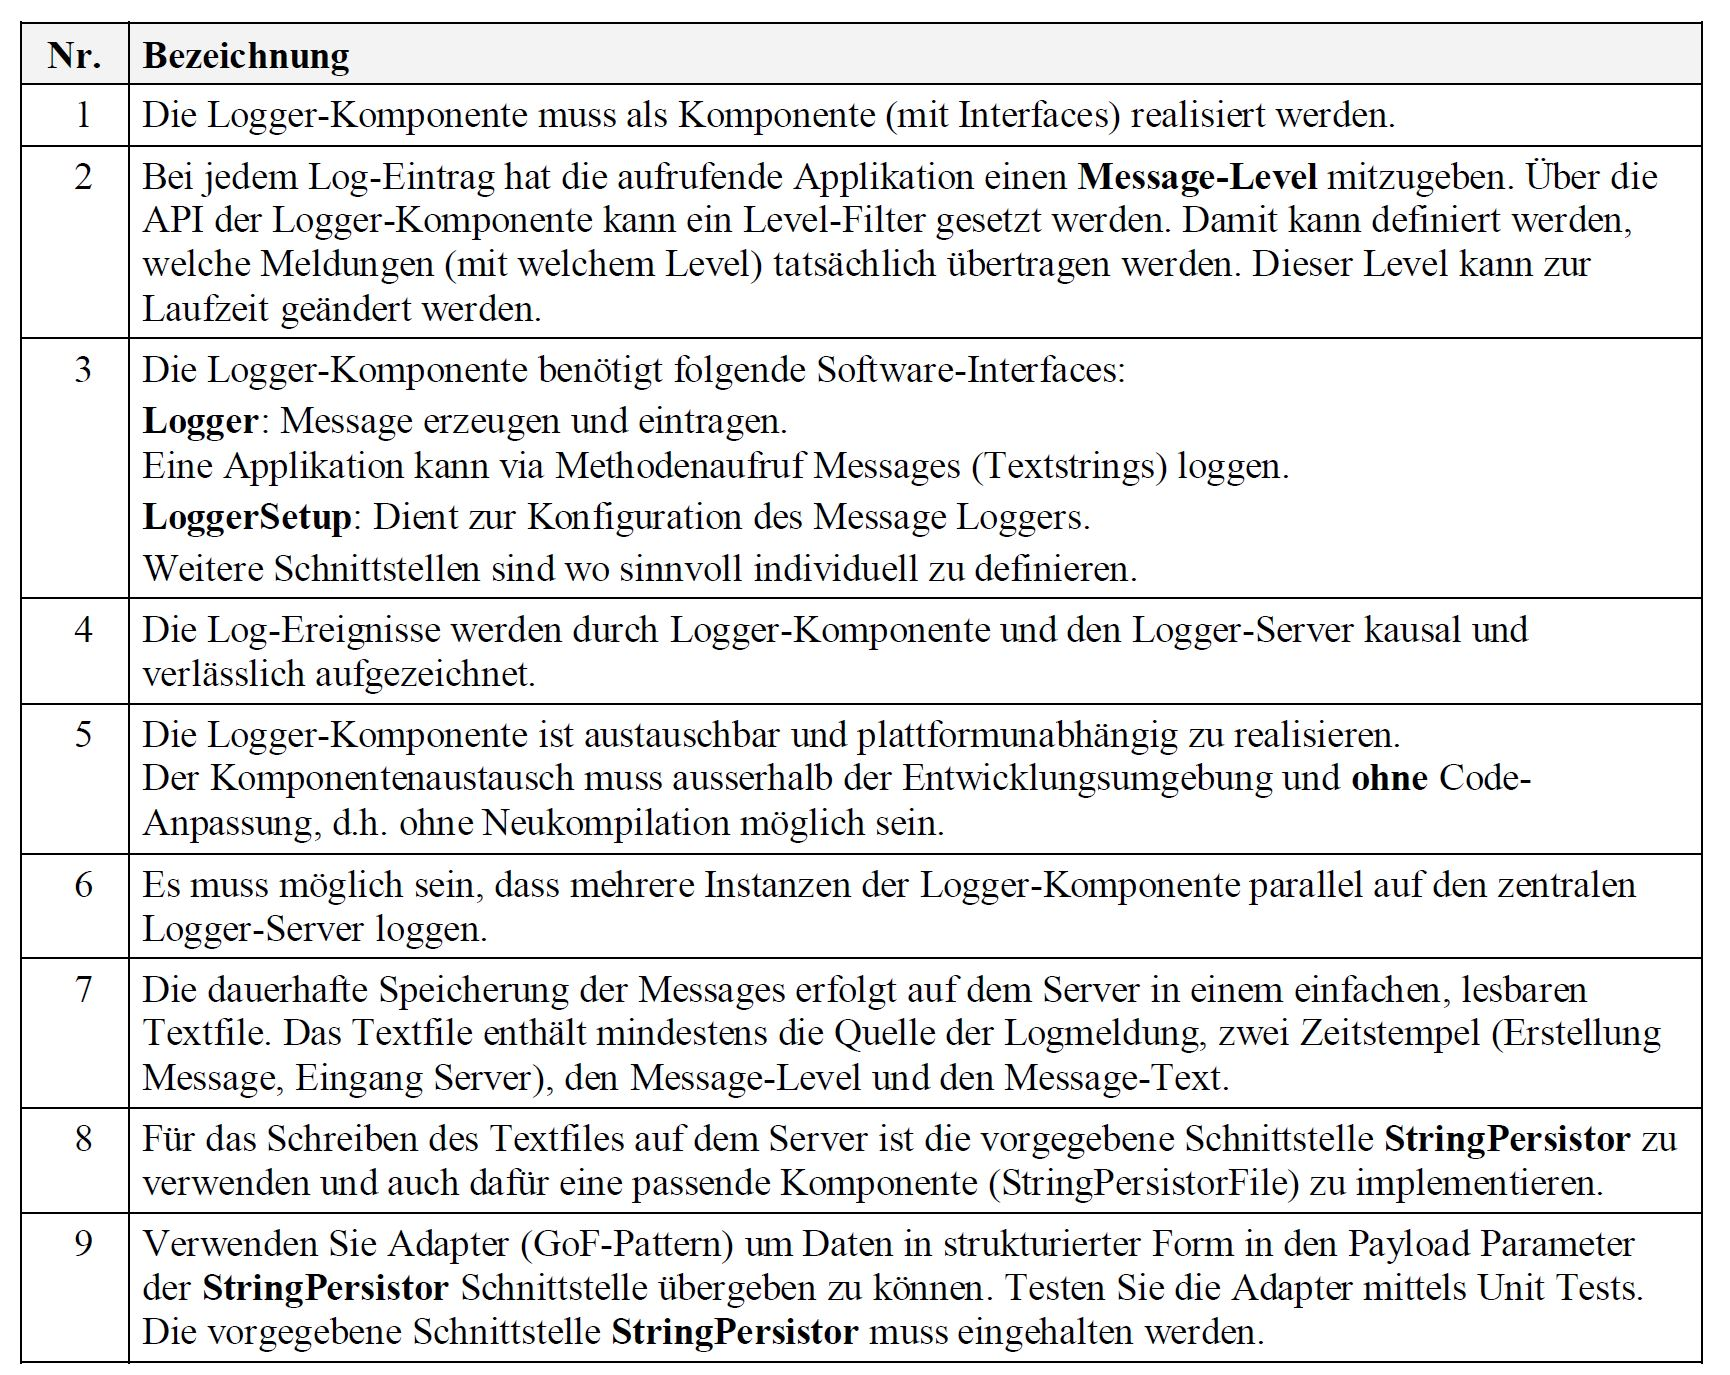
\includegraphics[height=9cm,keepaspectratio]{images/meilenstein1.JPG}
\end{center}

\paragraph{Meilensteinziele}
\begin{itemize}
	\itemsep0pt
	\item 1. Ein Logger-Interface zur Verfügung stellen
	\item 2. Logger-Komponente implementieren
	\item 3. Logger-Server implementieren
	\item 4. StringPersistor-Komponente implementieren
	\item 5. Events innerhalb von Game-of-Life über das Logger-Interface mit der Logger-Komponente auf dem	Logger-Server mittels StringPersistor loggen
	\item 6. Vollständige Dokumentation
\end{itemize}

\paragraph{Meilensteinzielerreichung}
\begin{itemize}
	\itemsep0pt
	\item 1. Ein Logger-Interface steht zur Verfügung
	\item 2. Logger-Komponente wurde implementiert
	\item 3. Logger-Server wurde implementiert
	\item 4. StringPersistor inkl. StringPersistorFile wurde implementiert
	\item 5. Events innerhalb von Game-of-Life werden auf dem Logger-Server geloggt
	\item 6. Die Dokumentation ist vollständig
\end{itemize}


\subsubsection{Meilensteinbericht 3}

\paragraph{Termin Meilenstein 3}
Die dritte Meilenstein findet zu Beginn der vierzehnten Semesterwoche statt.

\paragraph{Beschreibung Meilenstein 3}
Beim dritten Meilenstein geht es um den zweiten und finalen Release des Projektes. Es muss eine Demo des
Message Logging Systems vorgeführt werden. Die Programme des Systems müssen ausserhalb der
IDE lauffähig sein, in den vorgegebenen Projekten auf GitLab verwaltet werden, auf dem Buildserver
laufend integriert worden sein, automatisierte Tests ohne Fehler durchlaufen können und eine
begründete minimale Codeabdeckung erfüllen. Zudem muss eine vollständige Dokumentation
abgeliefert werden. Zudem müssen Komponenten zwischen den Teams ausgetauscht werden können.

\paragraph{Anforderungen an das Message Logging System}
\begin{center}
	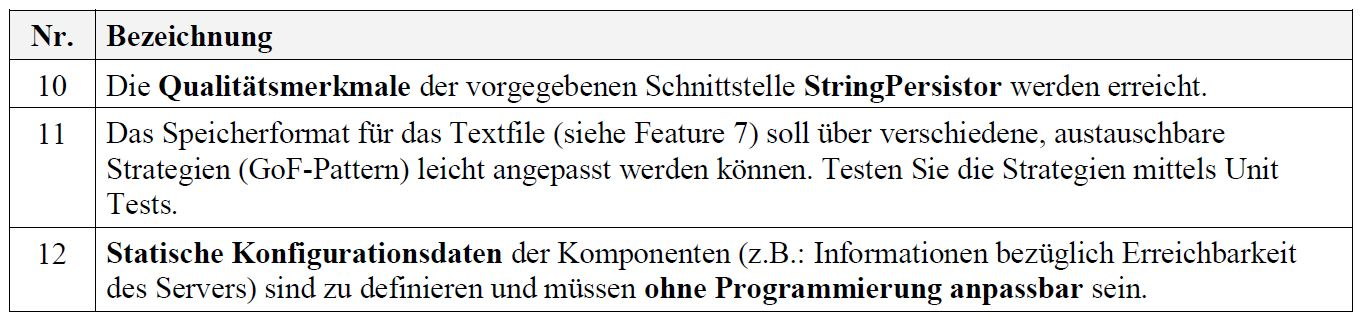
\includegraphics[height=4cm,keepaspectratio]{images/meilenstein2.1.JPG}
\end{center}
\begin{center}
	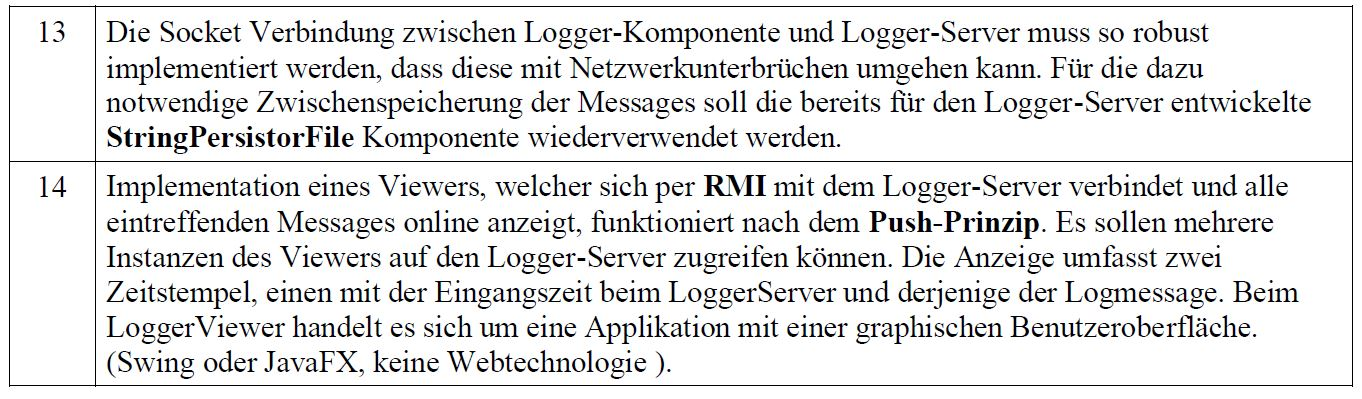
\includegraphics[height=5cm,keepaspectratio]{images/meilenstein2.2.JPG}
\end{center}

\paragraph{Meilensteinziele}
\begin{itemize}
	\itemsep0pt
	\item 1. StringPersistor soll Qualitätsmerkmale erfüllen
	\item 2. Strategy-Pattern implementieren
	\item 3. Client Lokaler-Logger implementieren
	\item 4. RMI implementieren

\end{itemize}

\paragraph{Meilensteinzielerreichung}
\begin{itemize}
	\itemsep0pt
	\item 1. StringPersistor erfüllt Qualitätsmerkmal
	\item 2. Strategy-Pattern wurde implementiert
	\item 3. Client Lokaler-Logger wurde implementiert
	\item 4. RMI wurde implementiert

\end{itemize}


\end{document}
